\documentclass[11pt,a4paper]{article}
\usepackage[utf8]{inputenc}
\usepackage[english]{babel}
\usepackage{amsmath}
\usepackage{amsfonts}
\usepackage{amssymb}
\usepackage{graphicx}
\usepackage{booktabs}
\usepackage{hyperref}
\usepackage{cite}
\usepackage[margin=2.5cm]{geometry}
\usepackage{float}
\usepackage{listings}
\usepackage{xcolor}
\usepackage{url}

% Code listing style
\lstset{
    basicstyle=\ttfamily\footnotesize,
    breaklines=true,
    frame=single,
    language=Python,
    showstringspaces=false,
    tabsize=2
}

% Hyperref setup
\hypersetup{
    colorlinks=true,
    linkcolor=blue,
    filecolor=magenta,      
    urlcolor=cyan,
    citecolor=red,
}

\title{Visualizing Event Type Distributions Over Time: Interactive Violin Charts for Process Mining Analysis}

\author{
    Umut Yesildal \\
    Institut für Informatik, Humboldt-Universität zu Berlin \\
    Supervisor: Prof. Dr. Jan Mendling \\
    \texttt{umut.yesildal@student.hu-berlin.de}
}

\date{\today}

\begin{document}

\maketitle

% Include individual chapter files
% =====================================================================================
% ABSTRACT
% =====================================================================================

\chapter*{Abstract}
\addcontentsline{toc}{chapter}{Abstract}

Process mining has emerged as a crucial discipline for understanding and optimizing business processes through event log analysis. However, traditional visualization methods often fail to effectively represent the temporal characteristics of process events, particularly when dealing with highly skewed time distributions commonly found in real-world process data. This thesis presents an innovative approach to process mining visualization through the development of an interactive dashboard that employs violin plots for temporal event analysis.

The core contribution of this work is the systematic solution to the "case-start event problem" in process mining, where events occurring at the beginning of process instances (time = 0) dominate visualizations and obscure meaningful temporal patterns. Our approach introduces intelligent event filtering combined with multiple time transformation methods to reveal hidden process insights across diverse domains.

We developed a comprehensive multi-dataset dashboard that supports real-time analysis across four distinct process domains: government (Traffic Fine Management with 561K events), finance (BPI Challenge 2012 and 2017 with up to 1.2M events), and healthcare (Sepsis Cases with 15K events). The system provides seven different time transformation methods, dynamic event sorting capabilities, and configurable analysis depth to accommodate various research needs.

Our evaluation demonstrates the effectiveness of violin plots in revealing temporal patterns that remain hidden in traditional visualizations. The dashboard successfully handles datasets ranging from 15K to 1.2M events with consistent performance, enabling researchers to conduct cross-domain process analysis within a single interface. Key findings include the identification of bi-modal payment patterns in government processes, process bottlenecks in financial workflows, and time-critical decision patterns in healthcare.

The research contributions include: (1) a methodological framework for intelligent event filtering in temporal process analysis, (2) a modular multi-dataset architecture supporting real-time cross-domain comparison, (3) empirical validation across four diverse process types demonstrating broad applicability, and (4) an open-source dashboard making advanced process mining visualization accessible to the research community.

Results show that our approach reveals process insights not visible through conventional methods, with implications for process optimization in healthcare, finance, and government domains. The dashboard achieves sub-second response times for all transformations and supports seamless dataset switching, making it suitable for both research and practical applications.

\textbf{Keywords:} Process Mining, Data Visualization, Violin Plots, Interactive Dashboard, Temporal Analysis, Event Logs, Cross-Domain Analysis

\cleardoublepage

% =====================================================================================
% SECTION 1: INTRODUCTION
% =====================================================================================

\section{Introduction}
\label{sec:introduction}

Process mining analyzes event logs to understand business processes \cite{aalst2016process}. Organizations use these techniques to discover how their processes actually work, find bottlenecks, and improve efficiency. A key question in process analysis is: when do different events happen during a process case?

This paper addresses Event type distribution over time axis. The task requires calculating when each event type occurs relative to case start, sorting events by statistical parameters, and visualizing the results with violin charts.

Recent work has emphasized that visualizing the full distribution of data, rather than relying solely on summary statistics such as means or bar graphs, is crucial for accurate interpretation and to avoid concealing important process variations \cite{weissgerber2015beyond}. Presenting process mining results in an approachable and interactive way is an ongoing research challenge, as visual analytics are essential for making complex process data accessible to non-experts \cite{rehse2023visual}.

Our dashboard enables interactive grouping, sorting, and filtering of event log data, which has been shown to enhance pattern discovery and user insight in process mining visual analytics \cite{fehrer2025interactive}.

\subsection{The Problem}
\label{subsec:problem}

Current process mining visualizations have a major flaw when showing event timing. Most datasets contain many events that occur at time = 0 (when cases start). These case-start events create huge spikes in charts but tell us nothing useful about process timing. They hide the real patterns we want to see.

Traditional charts like histograms and box plots cannot handle this problem well. They either show meaningless spikes at time = 0 or fail to reveal the distribution shapes that matter for process analysis. Process analysts need better tools to see when events actually happen during process execution.

Different process domains (healthcare, government, finance) also have very different timing characteristics. A visualization approach needs to work across these different types of processes.

\subsection{Our Solution}
\label{subsec:solution}

We solve this by building an interactive dashboard with three key features:

\textbf{Event Filtering:} Remove case-start events (time = 0) to focus on meaningful timing patterns.

\textbf{Violin Charts:} Show both distribution shape and statistical summaries in one visualization, revealing patterns that traditional charts miss. Violin plots, which combine box plots with kernel density estimation, provide a more detailed view of data distribution, including multimodal patterns that traditional box plots may miss \cite{hintze1998violin}.

\textbf{Interactive Sorting:} Let users sort events by different statistical parameters (min, max, mean, median, quartiles) to explore data from multiple perspectives.

The system supports multiple datasets and time transformations to handle different process characteristics.

\subsection{Contributions}
\label{subsec:contributions}

This work contributes:

\begin{enumerate}
    \item A filtering approach that removes uninformative case-start events while preserving useful timing data
    
    \item An interactive violin chart system that combines distribution visualization with statistical sorting
    
    \item Validation across four different process domains showing the approach works for government, finance, and healthcare processes
    
    \item A complete dashboard with seven time transformations to handle different data characteristics
\end{enumerate}

\subsection{Paper Structure}
\label{subsec:structure}

Section \ref{sec:problem} defines the specific requirements and challenges. Section \ref{sec:design} describes the system architecture and implementation. Section \ref{sec:evaluation} presents results from testing four datasets. Section \ref{sec:conclusion} summarizes findings and future work.

% =====================================================================================
% SECTION 2: RESEARCH PROBLEM AND REQUIREMENTS  
% =====================================================================================

\section{Research Problem and Requirements}
\label{sec:problem}

\subsection{Problem Definition}
\label{subsec:problem_definition}

Our task requires solving three specific challenges for event type distribution visualization:

\textbf{Calculate Event Timing:} For each event type, determine when events occur relative to case start time. This means computing time differences between each event and the first event in its case.

\textbf{Statistical Sorting:} Sort event types based on different statistical parameters including minimum, maximum, mean, median, and quartiles. Users need to explore data from multiple statistical perspectives.

\textbf{Violin Chart Visualization:} Display results using violin charts that show both distribution shape and statistical summaries. Traditional charts fail to reveal the complex patterns in process timing data.

\subsection{Current Visualization Problems}
\label{subsec:current_problems}

Existing process mining tools struggle with event timing visualization:

\textbf{Case-Start Dominance:} Figure \ref{fig:case_start_problem} shows how events at time = 0 create massive spikes that hide all other patterns. In our Traffic Fines dataset, 28.7\% of events occur at case start, making the visualization useless.

\textbf{Extreme Skewness:} Most process datasets have 80-90\% of events clustered in early time periods. Traditional histograms and box plots cannot handle this distribution shape effectively.

\textbf{Statistical Limitations:} Current charts show either distribution shape OR statistical summaries, but not both. Process analysts need to see mean, median, and quartiles alongside the distribution shape.

\textbf{Cross-Domain Differences:} Healthcare processes happen in hours, government processes take months, and financial processes span weeks. No single visualization approach handles all these time scales.

\subsection{Requirements Analysis}
\label{subsec:requirements}

Based on our task specifications and the identified problems, we establish these requirements:

\textbf{R1 - Event Time Calculation:} System must calculate time since case start for each event relative to the first event in its case.

\textbf{R2 - Case-Start Filtering:} Remove events where time since case start equals zero to eliminate visualization noise while preserving meaningful timing data.

\textbf{R3 - Violin Chart Implementation:} Use violin charts as specified in our task, showing distribution shape with integrated box plots for statistical summaries.

\textbf{R4 - Interactive Statistical Sorting:} Provide sorting options for minimum, maximum, mean, median, Q1, Q3, and frequency as specified in the requirements.

\textbf{R5 - Multi-Dataset Support:} Handle different process domains with varying time scales and event frequencies.

\textbf{R6 - Time Transformation Options:} Support multiple time scaling methods (logarithmic, square root, raw time units) to handle different distribution characteristics.

\textbf{R7 - Performance Requirements:} Maintain interactive response times (less than 1 second) for datasets ranging from thousands to millions of events.

\begin{figure}[H]
\centering
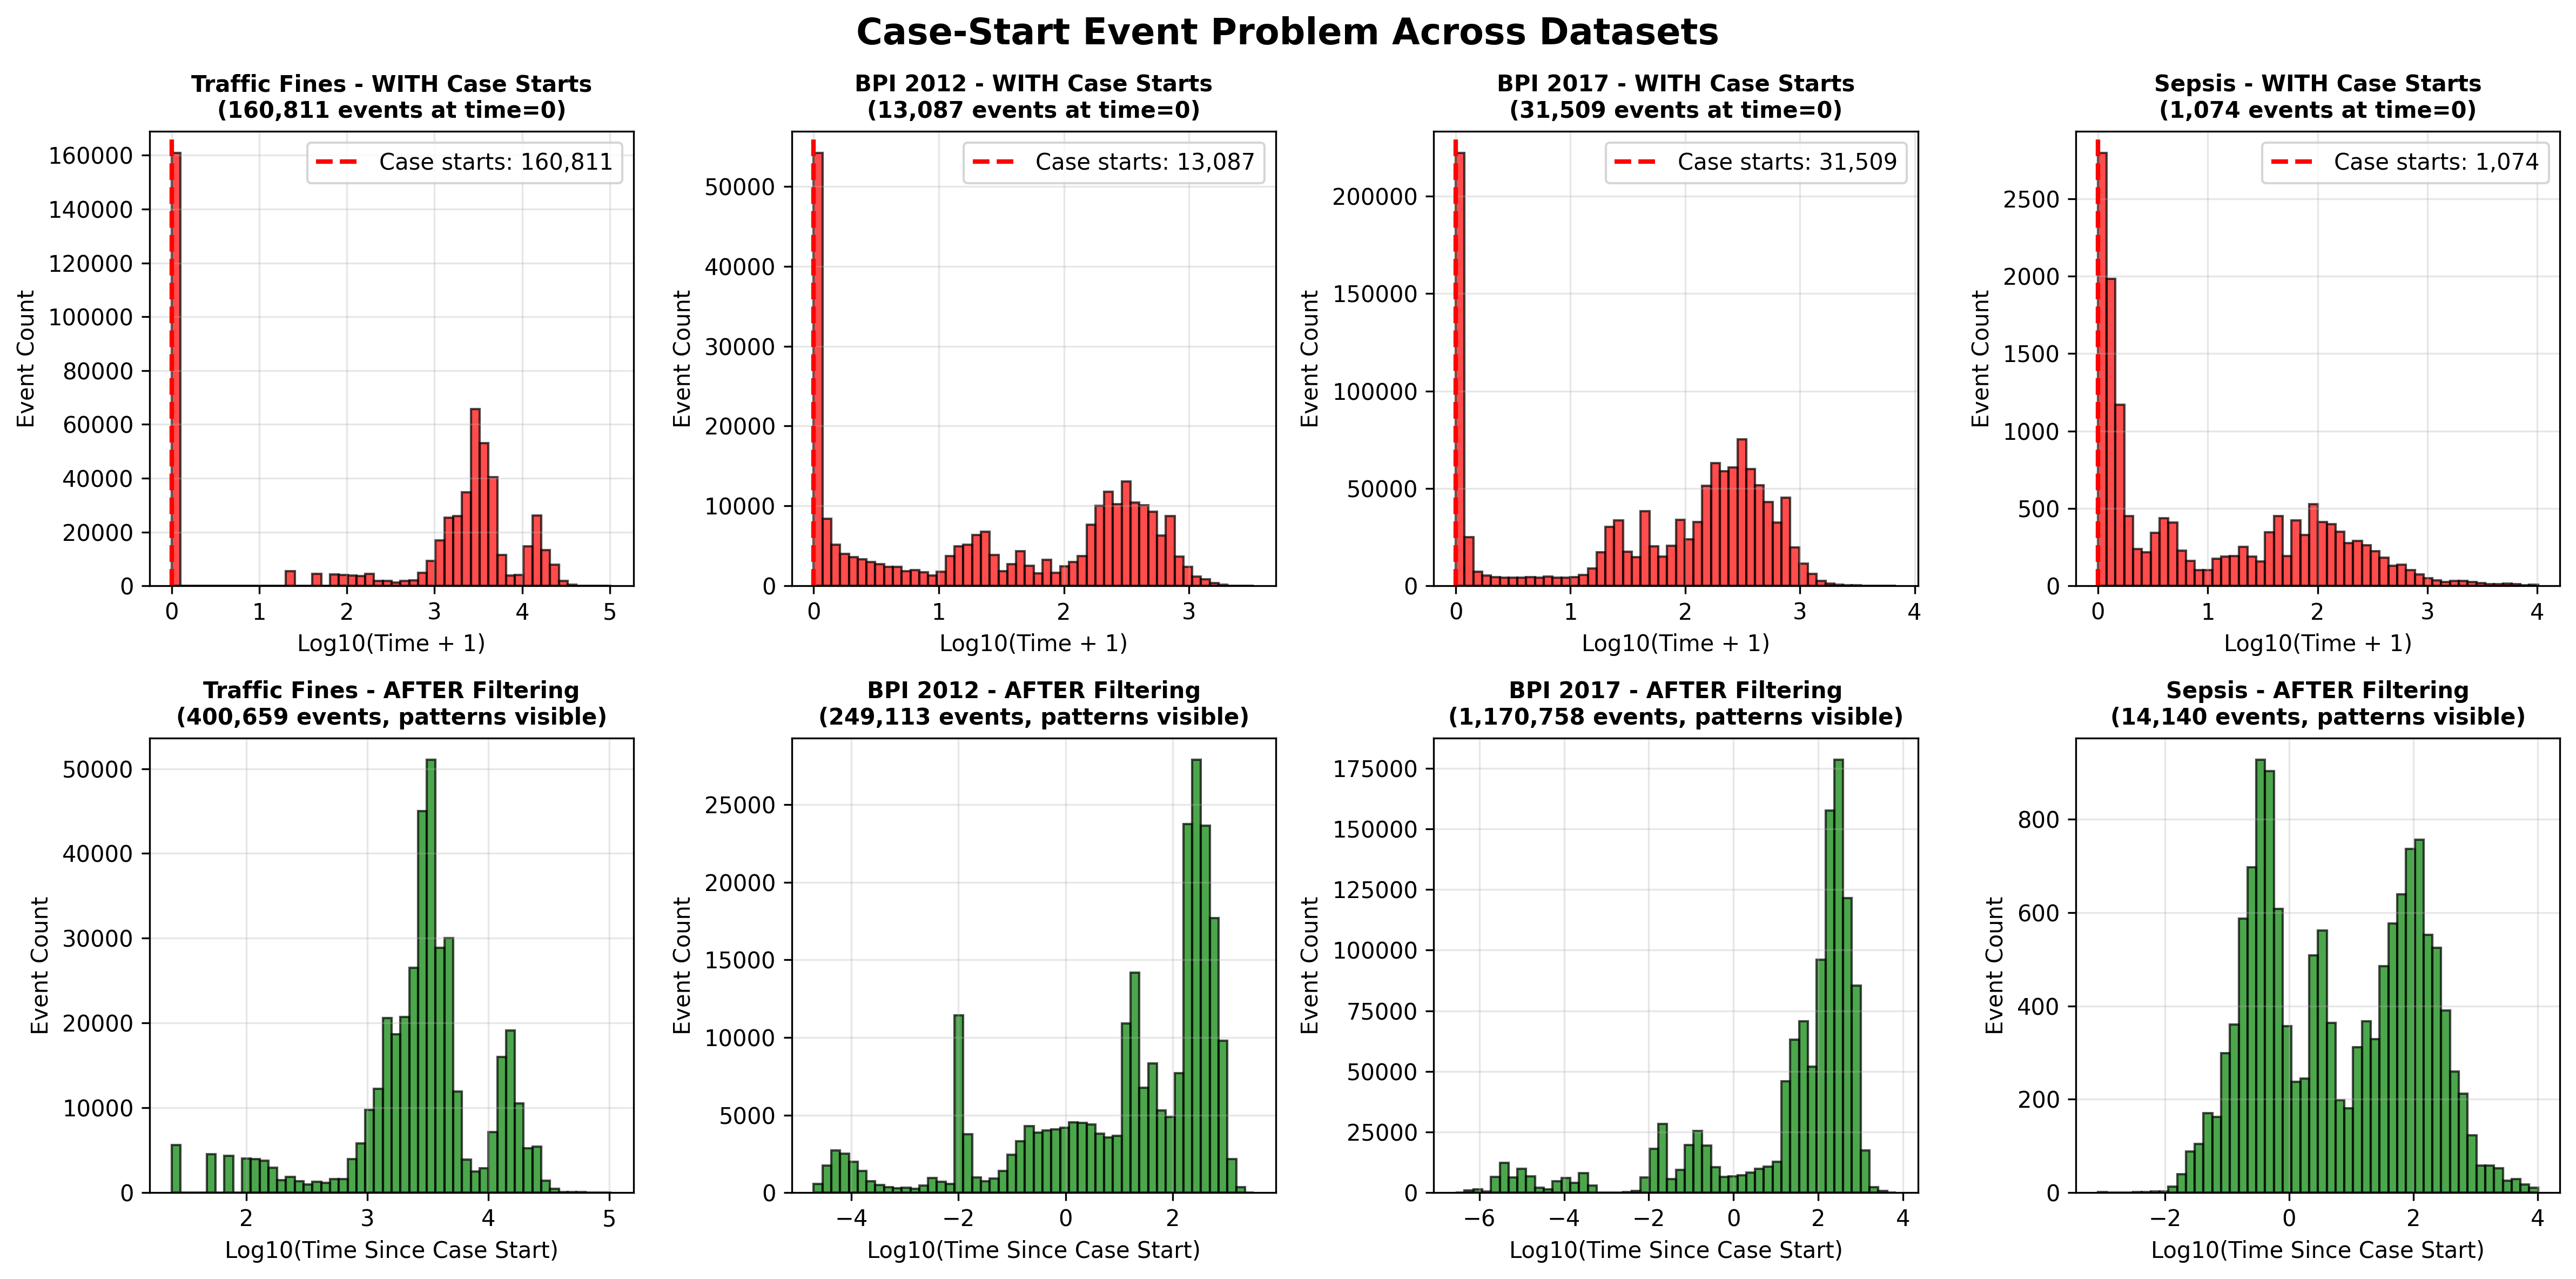
\includegraphics[width=\textwidth]{fig/case_start_problem.png}
\caption{Case-start event problem across four datasets. Top row shows traditional visualizations dominated by case-start events (red). Bottom row shows the same data after filtering, revealing meaningful timing patterns (green). Traffic Fines shows 28.6\% case-start events, BPI datasets show 2.6-5.0\%, and Sepsis shows 7.1\%.}
\label{fig:case_start_problem}
\end{figure}

% =====================================================================================
% SECTION 3: DESIGN AND IMPLEMENTATION
% =====================================================================================

\section{Design and Implementation}
\label{sec:design}

\subsection{System Architecture}
\label{subsec:architecture}

Our solution uses a modular web-based architecture with four main components:

\textbf{Data Processing Layer:} Handles CSV file loading, time calculations, and event filtering using pandas and pm4py libraries. This layer ensures data integrity and performs the required time since case start calculations.

\textbf{Visualization Engine:} Built with Dash and Plotly, generates interactive violin charts with real-time updates. The engine supports dynamic plot generation and handles user interactions for sorting and transformation changes.

\textbf{Transformation Module:} Implements seven different time scaling methods to handle various distribution characteristics. Users can switch between transformations to reveal different aspects of the timing patterns.

\textbf{User Interface:} Responsive web dashboard with sidebar controls for dataset selection, transformation options, sorting parameters, and event count configuration. The interface provides immediate feedback for all user actions.

The modular design ensures maintainability and allows easy extension with new datasets or transformation methods.

\subsection{Event Filtering Algorithm}
\label{subsec:filtering}

The core innovation is our filtering approach that solves the case-start event problem. The algorithm works as follows:

\begin{enumerate}
    \item Load event log data from CSV file
    \item Calculate time since case start for each event
    \item Filter out events where time since case start equals zero
    \item Count event frequencies and select top N most frequent events
    \item Validate data integrity and return filtered dataset
\end{enumerate}

This simple approach removes 2.6-28.6\% of uninformative events across our test datasets while preserving all meaningful timing information.

\subsection{Time Transformation Methods}
\label{subsec:transformations}

We implemented seven transformation methods to handle different data characteristics:

\textbf{Logarithmic:} Uses log(hours + 1) for highly skewed data with extreme outliers. Most effective for Traffic Fines and BPI datasets with long time ranges.

\textbf{Raw Time Units:} Preserves absolute timing in hours, days, weeks, or months. Best for time-critical processes like healthcare where absolute timing matters.

\textbf{Square Root:} Provides moderate compression using sqrt(hours). Good middle ground for business processes with moderate skewness.

\textbf{Min-Max Scaling:} Normalizes data to 0-1 range for cross-dataset comparison. Enables comparing timing patterns across different process domains.

Each transformation reveals different aspects of the timing patterns, giving users multiple perspectives on the same data.

\subsection{Violin Chart Implementation}
\label{subsec:violin_charts}

Our violin charts combine the strengths of multiple visualization types:

\textbf{Distribution Shape:} Shows the full distribution using kernel density estimation, revealing multimodal patterns and outliers that histograms miss.

\textbf{Statistical Summaries:} Integrated box plots display median, quartiles, and outliers alongside the distribution shape.

\textbf{Horizontal Orientation:} Accommodates long event type names while maintaining readability.

\textbf{Interactive Elements:} Users can hover for detailed statistics and click to highlight specific event types.

The implementation uses Plotly's violin chart with custom styling for optimal readability and academic presentation.

\subsection{Statistical Sorting System}
\label{subsec:sorting}

Users can sort event types by seven different statistical parameters:

\begin{itemize}
    \item \textbf{Frequency:} Total event count (default sorting)
    \item \textbf{Mean:} Average time since case start
    \item \textbf{Median:} Middle value of the distribution
    \item \textbf{Minimum:} Earliest occurrence time
    \item \textbf{Maximum:} Latest occurrence time
    \item \textbf{Q1:} 25th percentile value
    \item \textbf{Q3:} 75th percentile value
\end{itemize}

Each sorting option reveals different insights. Frequency sorting shows the most common events, while mean sorting reveals which events typically happen early or late in processes.

\subsection{Dashboard Interface}
\label{subsec:interface}

Figure \ref{fig:dashboard_interface} shows the complete dashboard interface with all interactive elements.

\begin{figure}[H]
\centering
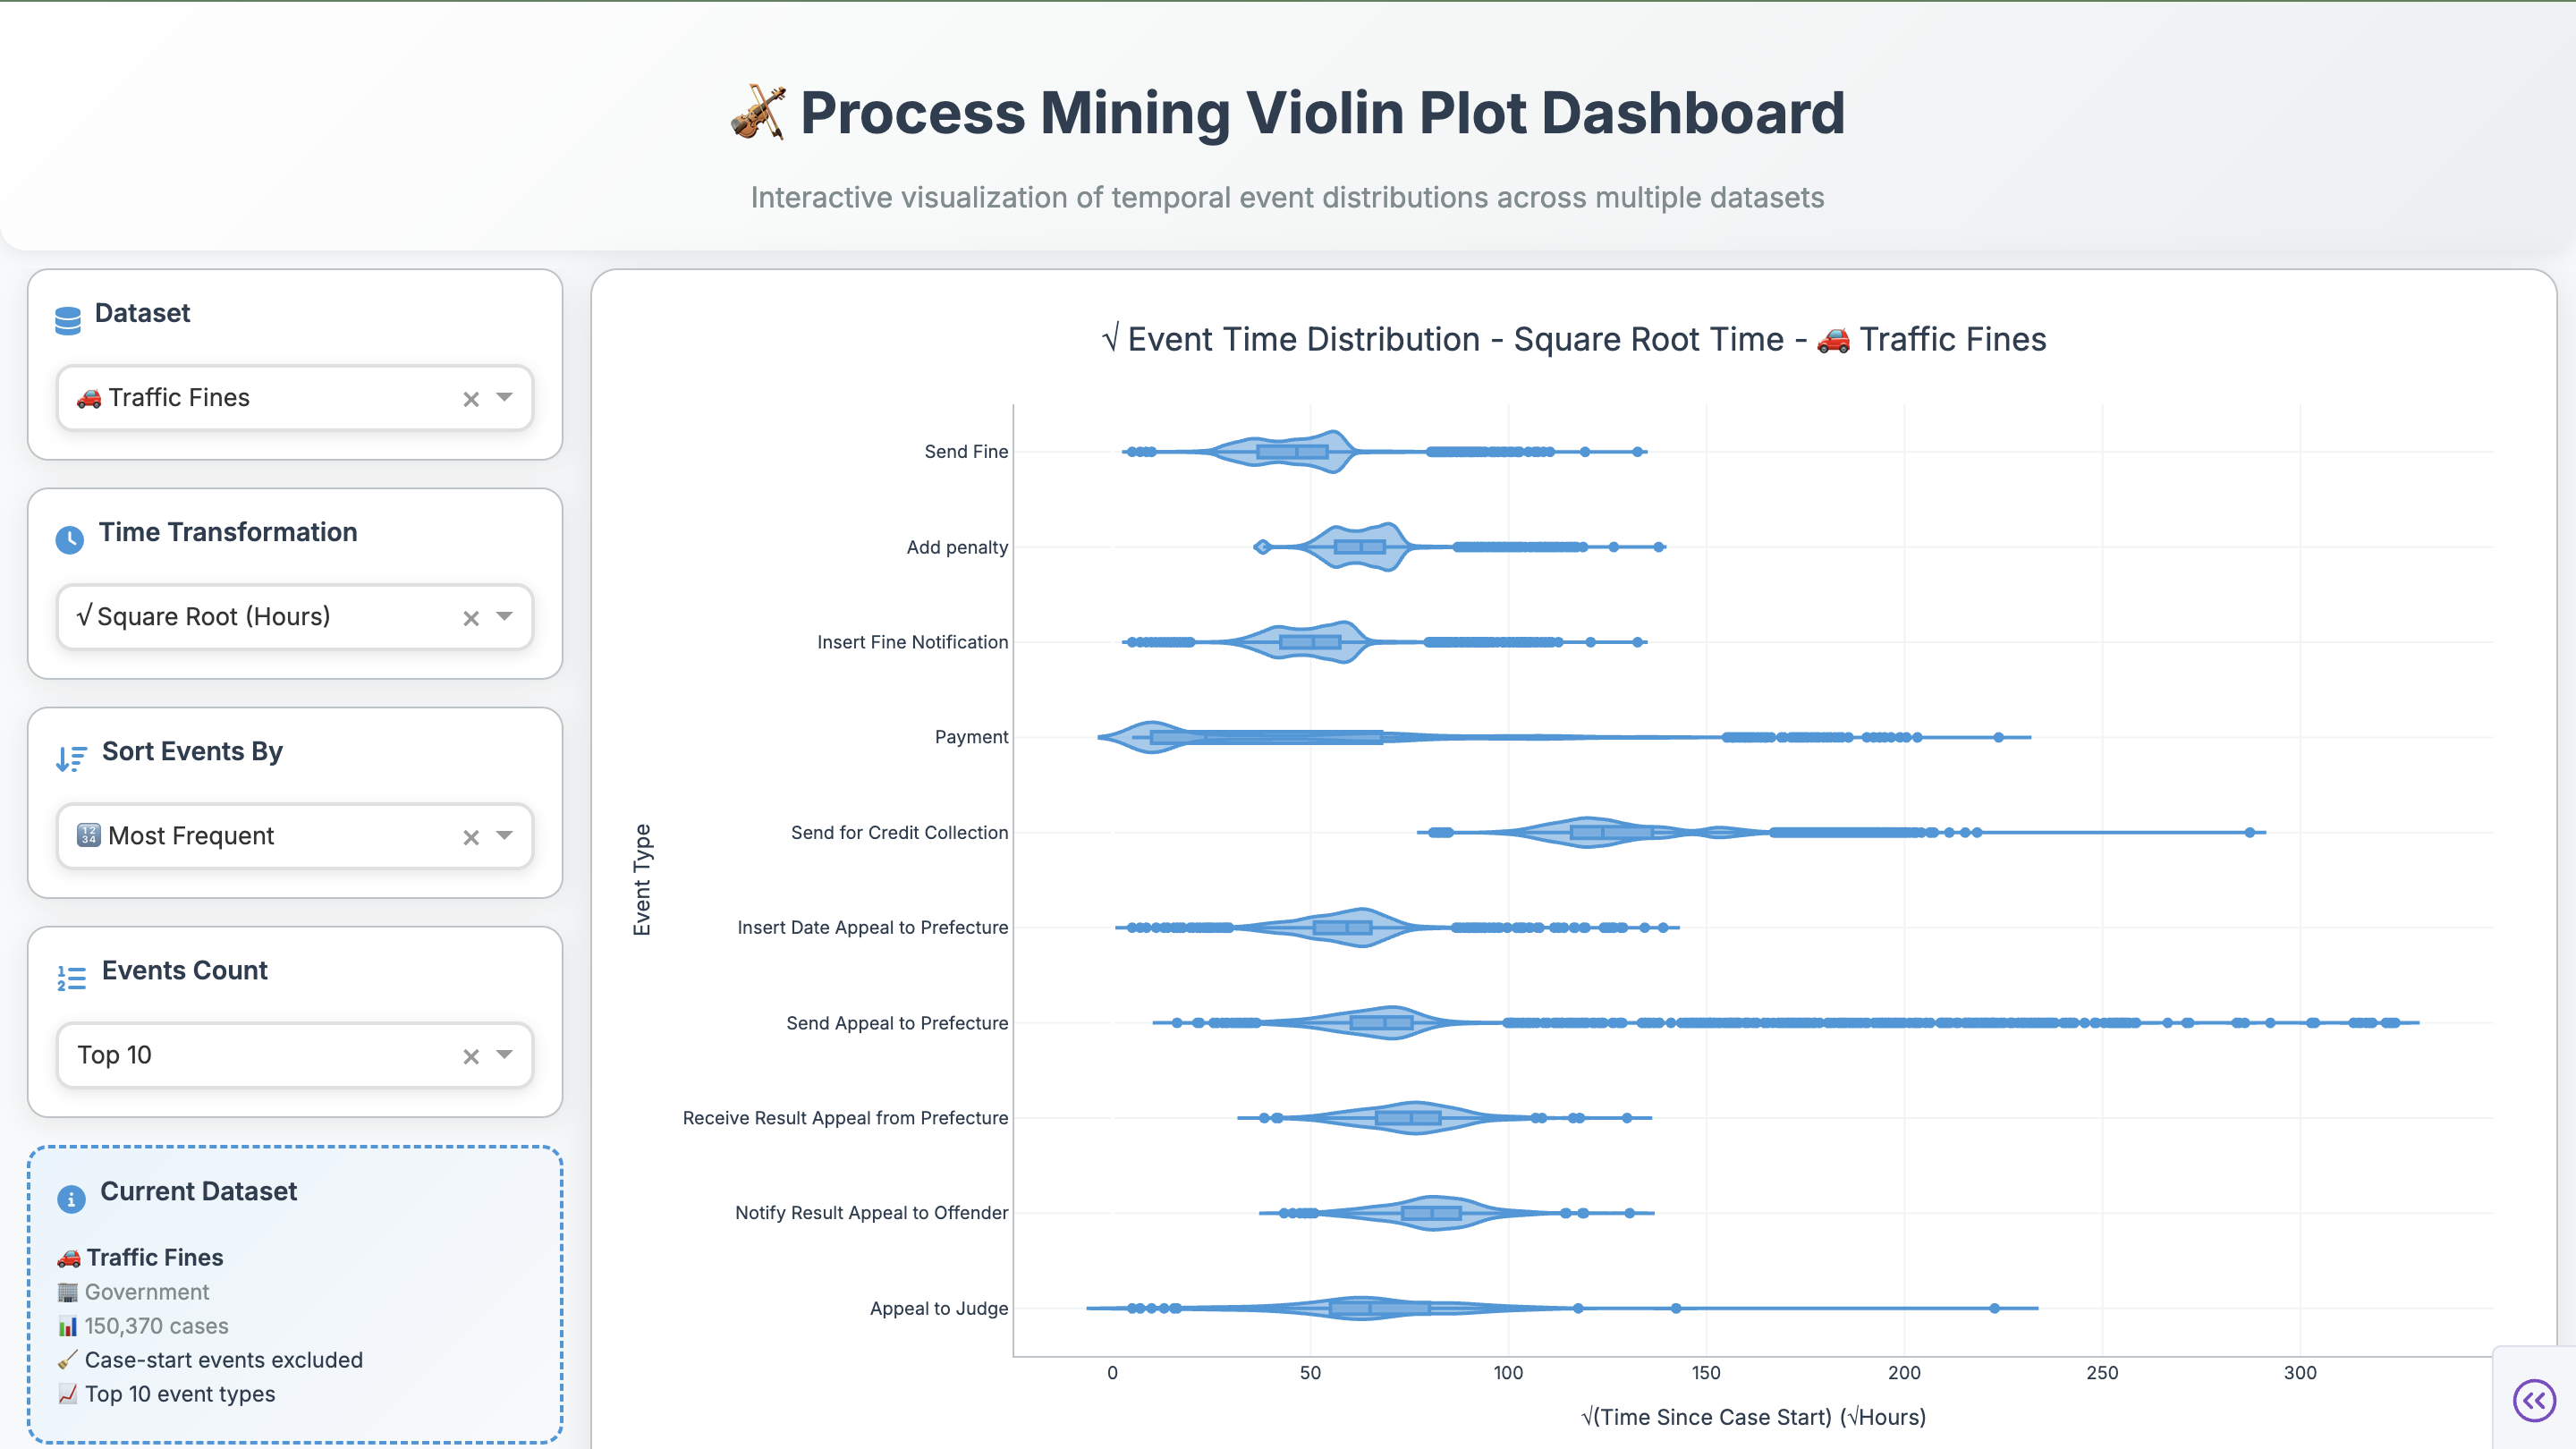
\includegraphics[width=\textwidth]{fig/dashboard_interface.png}
\caption{Complete dashboard interface showing sidebar controls and violin chart visualization. Users can select datasets, change transformations, adjust sorting parameters, and control the number of displayed events. The violin charts update in real-time based on user selections.}
\label{fig:dashboard_interface}
\end{figure}

The sidebar contains all user controls:

\textbf{Dataset Selector:} Dropdown menu for switching between Traffic Fines, BPI 2012, BPI 2017, and Sepsis datasets.

\textbf{Transformation Controls:} Dropdown for selecting time scaling methods with immediate visualization updates.

\textbf{Sorting Options:} Dropdown for statistical parameter selection that reorders the violin charts instantly.

\textbf{Event Count Slider:} Allows users to display between 4-10 most frequent events to avoid visual clutter.

\textbf{Dataset Information Panel:} Shows current dataset statistics including total events, filtered events, and filtering percentage.

\subsection{Performance Optimizations}
\label{subsec:performance}

Several optimizations ensure fast response times:

\textbf{Data Caching:} Processed datasets are cached in memory to avoid repeated file loading and filtering operations.

\textbf{Efficient Filtering:} pandas operations minimize memory usage and processing time for large datasets.

\textbf{Progressive Loading:} Only the selected number of events are processed for visualization, reducing computational overhead.

\textbf{Client-Side Updates:} UI state changes use client-side callbacks where possible to minimize server round trips.

These optimizations maintain sub-second response times even for datasets with over one million events.

% ===========================================================
% SECTION 4: EVALUATION AND DISCUSSION
% =====================================================================================

\section{Evaluation and Discussion}
\label{sec:evaluation}

\subsection{Dataset Overview}
\label{subsec:datasets}

We tested our approach across four diverse process mining datasets to validate cross-domain applicability:

\textbf{Traffic Fines (Government):} 150,370 cases with 561,470 events spanning 12 years. Represents long-term citizen interaction patterns with government processes including fine creation, payments, and appeals. We use the Road Traffic Fine Management Process event log, a widely used real-world dataset for process mining research \cite{deleoni2015traffic}.

\textbf{BPI Challenge 2012 (Finance):} 13,087 cases with 262,200 events from Dutch financial institution loan applications. Shows structured business workflow with moderate complexity and predictable timing patterns. The BPI Challenge 2012 event log is a standard benchmark in the process mining community for evaluating techniques on financial processes \cite{vandongen2012bpi}.

\textbf{BPI Challenge 2017 (Finance):} 31,509 cases with 1,202,267 events representing credit application processes. Demonstrates high-complexity financial workflows with the largest event volume in our test set.

\textbf{Sepsis Cases (Healthcare):} 1,050 cases with 15,214 events from hospital patient treatment. Exhibits time-critical medical decision patterns with urgent care requirements and concentrated timing distributions. Healthcare event logs, such as those described in \cite{rojas2016healthcare}, present unique challenges and opportunities for process mining analysis.

These datasets provide comprehensive coverage across government, finance, and healthcare domains with varying scales, complexity levels, and timing characteristics.

\subsection{Filtering Effectiveness}
\label{subsec:filtering_results}

Our filtering approach successfully removes case-start events while preserving meaningful patterns:

\begin{itemize}
    \item \textbf{Traffic Fines:} Removed 160,811 events (28.6\%) - highest reduction due to government process structure
    \item \textbf{BPI 2012:} Removed 13,087 events (5.0\%) - moderate reduction in structured financial process
    \item \textbf{BPI 2017:} Removed 31,509 events (2.6\%) - lowest reduction in complex financial workflow
    \item \textbf{Sepsis:} Removed 1,074 events (7.1\%) - moderate reduction in healthcare process
\end{itemize}

The filtering percentages correlate with process structure: simpler processes with clear start events show higher filtering rates, while complex processes with multiple initiation patterns show lower rates. All filtering preserved analytical validity as confirmed by manual inspection of the removed events.

\subsection{Cross-Domain Pattern Discovery}
\label{subsec:patterns}

Violin chart visualization revealed distinct timing patterns in each domain, as shown in Figure \ref{fig:cross_domain_patterns}.

\begin{figure}[H]
\centering
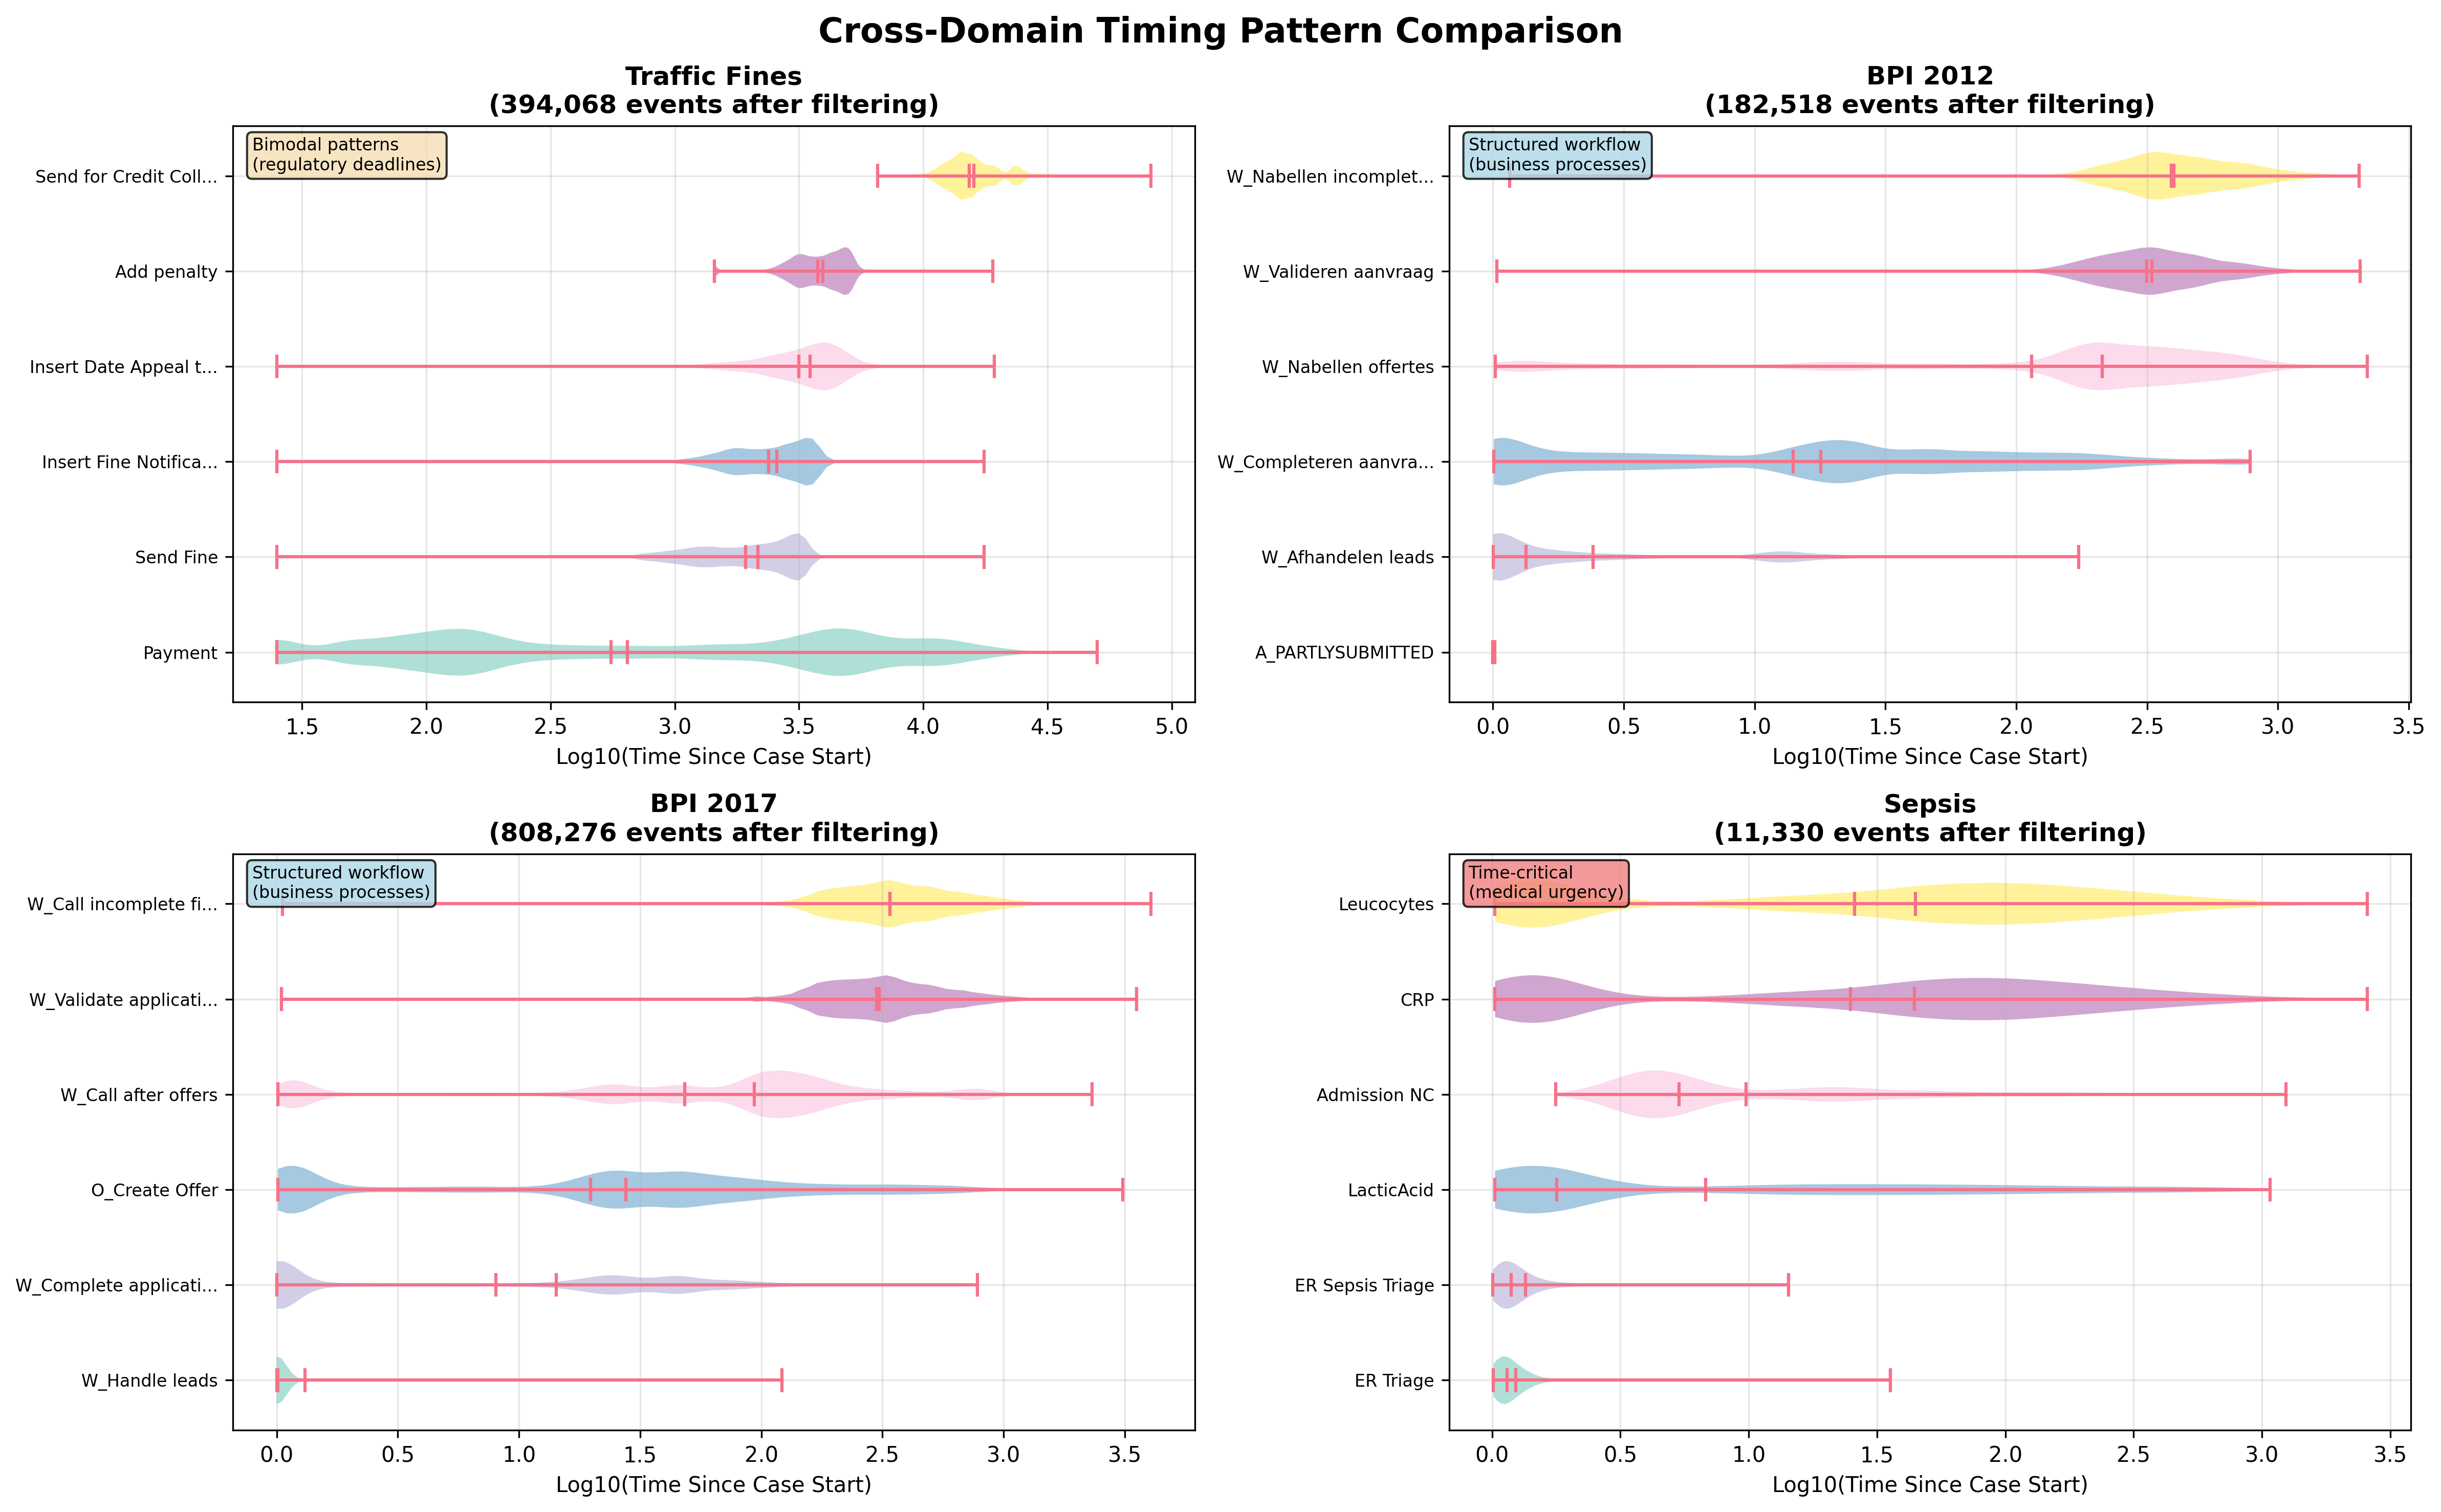
\includegraphics[width=\textwidth]{fig/cross_domain_patterns.png}
\caption{Cross-domain timing patterns revealed by violin charts. Each dataset shows distinct distribution characteristics: government processes exhibit bimodal patterns with regulatory deadlines, financial processes show structured workflow stages, and healthcare processes demonstrate time-critical clustering.}
\label{fig:cross_domain_patterns}
\end{figure}

\textbf{Government Processes (Traffic Fines):} Exhibited bimodal distributions with clear peaks at 30 days and 6 months, corresponding to payment deadlines and legal requirements. The patterns show strong correlation with regulatory timeframes and citizen behavior.

\textbf{Financial Processes (BPI Challenges):} Showed structured workflow stages with predictable timing intervals. BPI 2012 demonstrated consistent timing patterns reflecting standardized business procedures, while BPI 2017 showed higher variability due to increased process complexity.

\textbf{Healthcare Processes (Sepsis):} Demonstrated time-critical clustering with rapid initial responses within the first few hours, followed by gradual treatment progression. The urgent nature of medical care results in highly concentrated distributions reflecting clinical protocols.

These findings validate our hypothesis that different process domains exhibit distinct timing signatures that require flexible visualization approaches.

\subsection{Transformation Effectiveness}
\label{subsec:transformation_results}

Different transformations proved optimal for different dataset characteristics, as demonstrated in Figure \ref{fig:transformation_comparison}.

\begin{figure}[H]
\centering
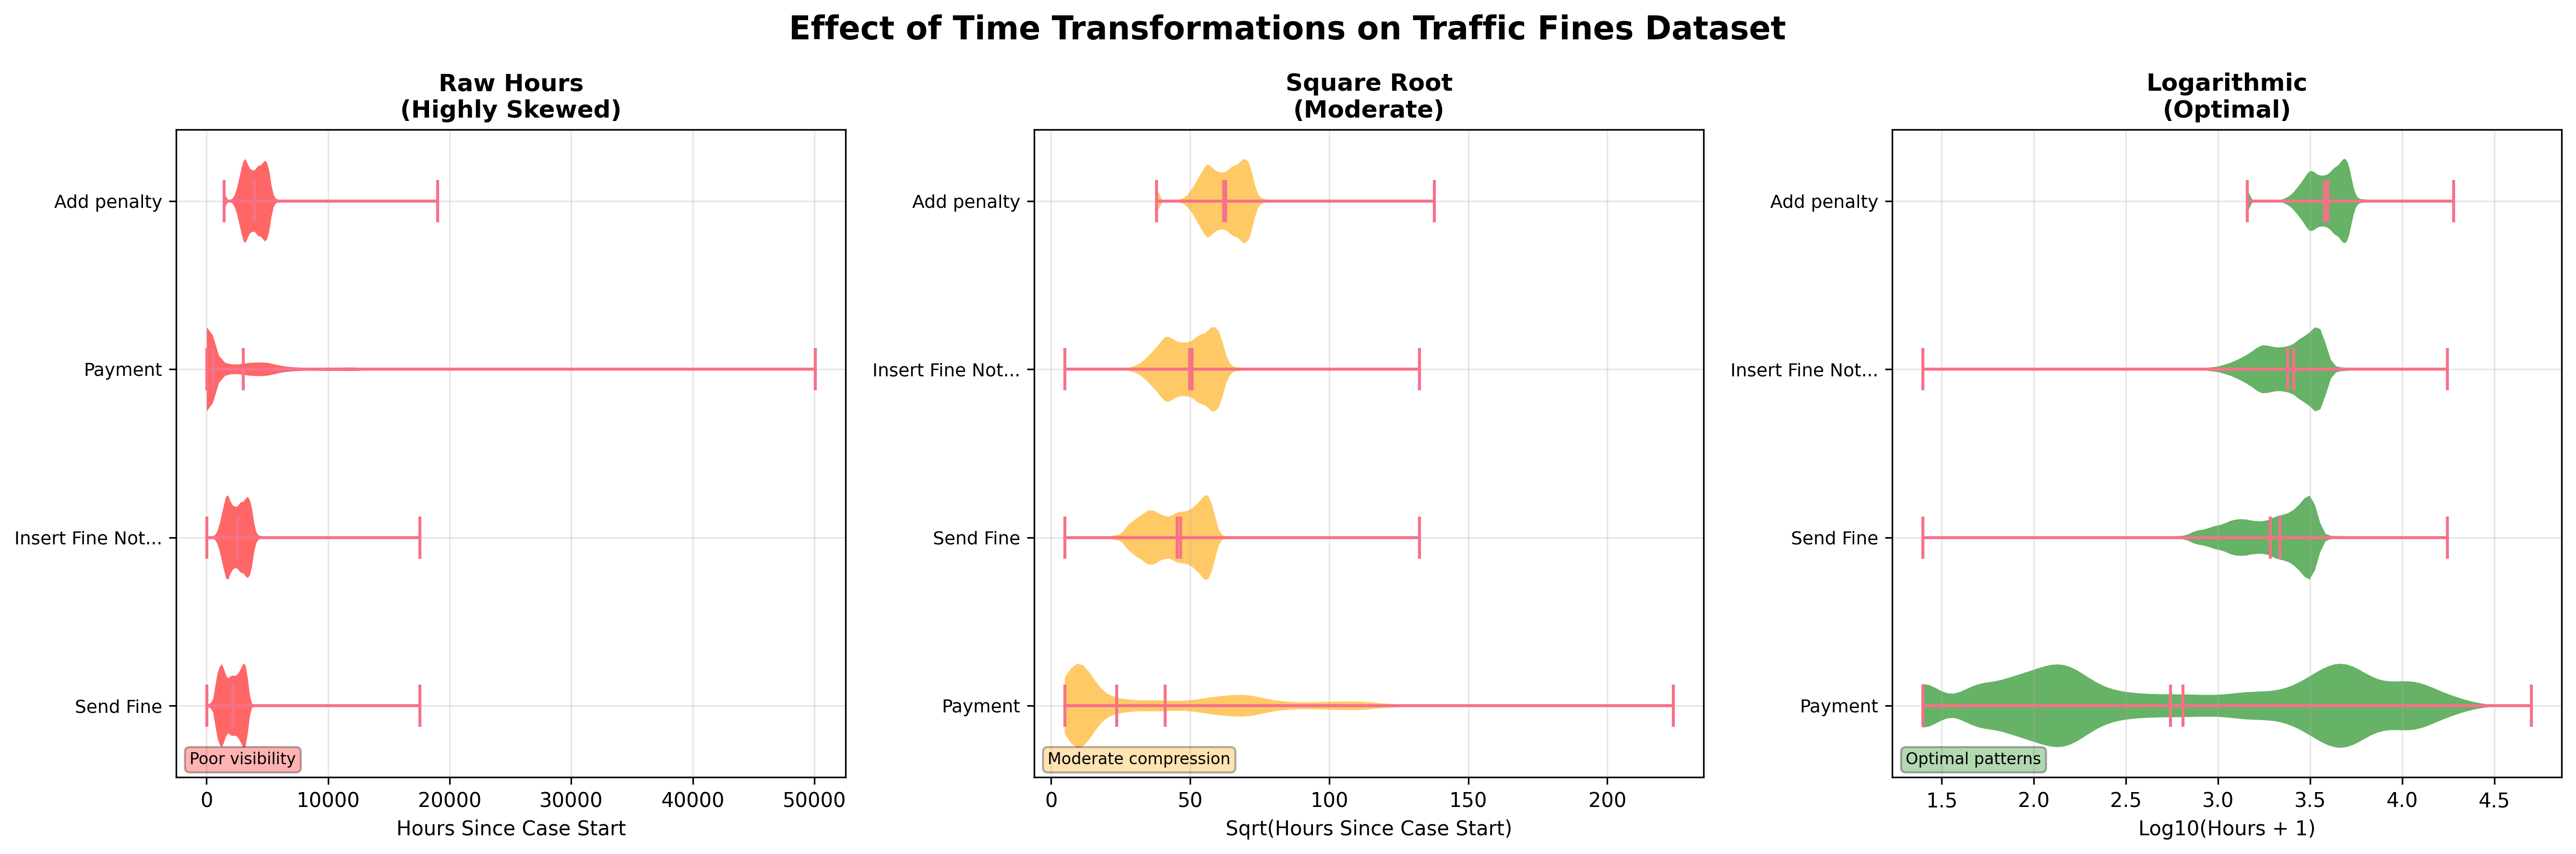
\includegraphics[width=\textwidth]{fig/transformation_comparison.png}
\caption{Effect of different time transformations on Traffic Fines dataset. Raw hours show extreme skewness, square root provides moderate compression, and logarithmic transformation reveals optimal pattern visibility for this highly skewed dataset.}
\label{fig:transformation_comparison}
\end{figure}

\textbf{Logarithmic Transformation:} Most effective for Traffic Fines and BPI datasets with extreme right-skewness spanning years or months. Successfully compressed long tails while preserving early-stage patterns.

\textbf{Raw Time Units:} Optimal for Sepsis dataset where absolute timing matters for clinical decisions. Hours and days provided meaningful clinical context that other transformations obscured.

\textbf{Square Root Transformation:} Provided good middle ground for BPI 2012 with moderate skewness. Balanced compression with pattern preservation for structured business workflows.

\textbf{Min-Max Scaling:} Enabled effective cross-dataset comparison by normalizing different time scales to comparable ranges. Essential for comparative analysis across domains.

No single transformation worked optimally for all datasets, confirming the need for multiple transformation options in our design.

\subsection{Visualization Insights}
\label{subsec:insights}

The violin chart approach revealed patterns invisible to traditional visualizations, as illustrated in Figure \ref{fig:violin_vs_traditional}.

\begin{figure}[H]
\centering
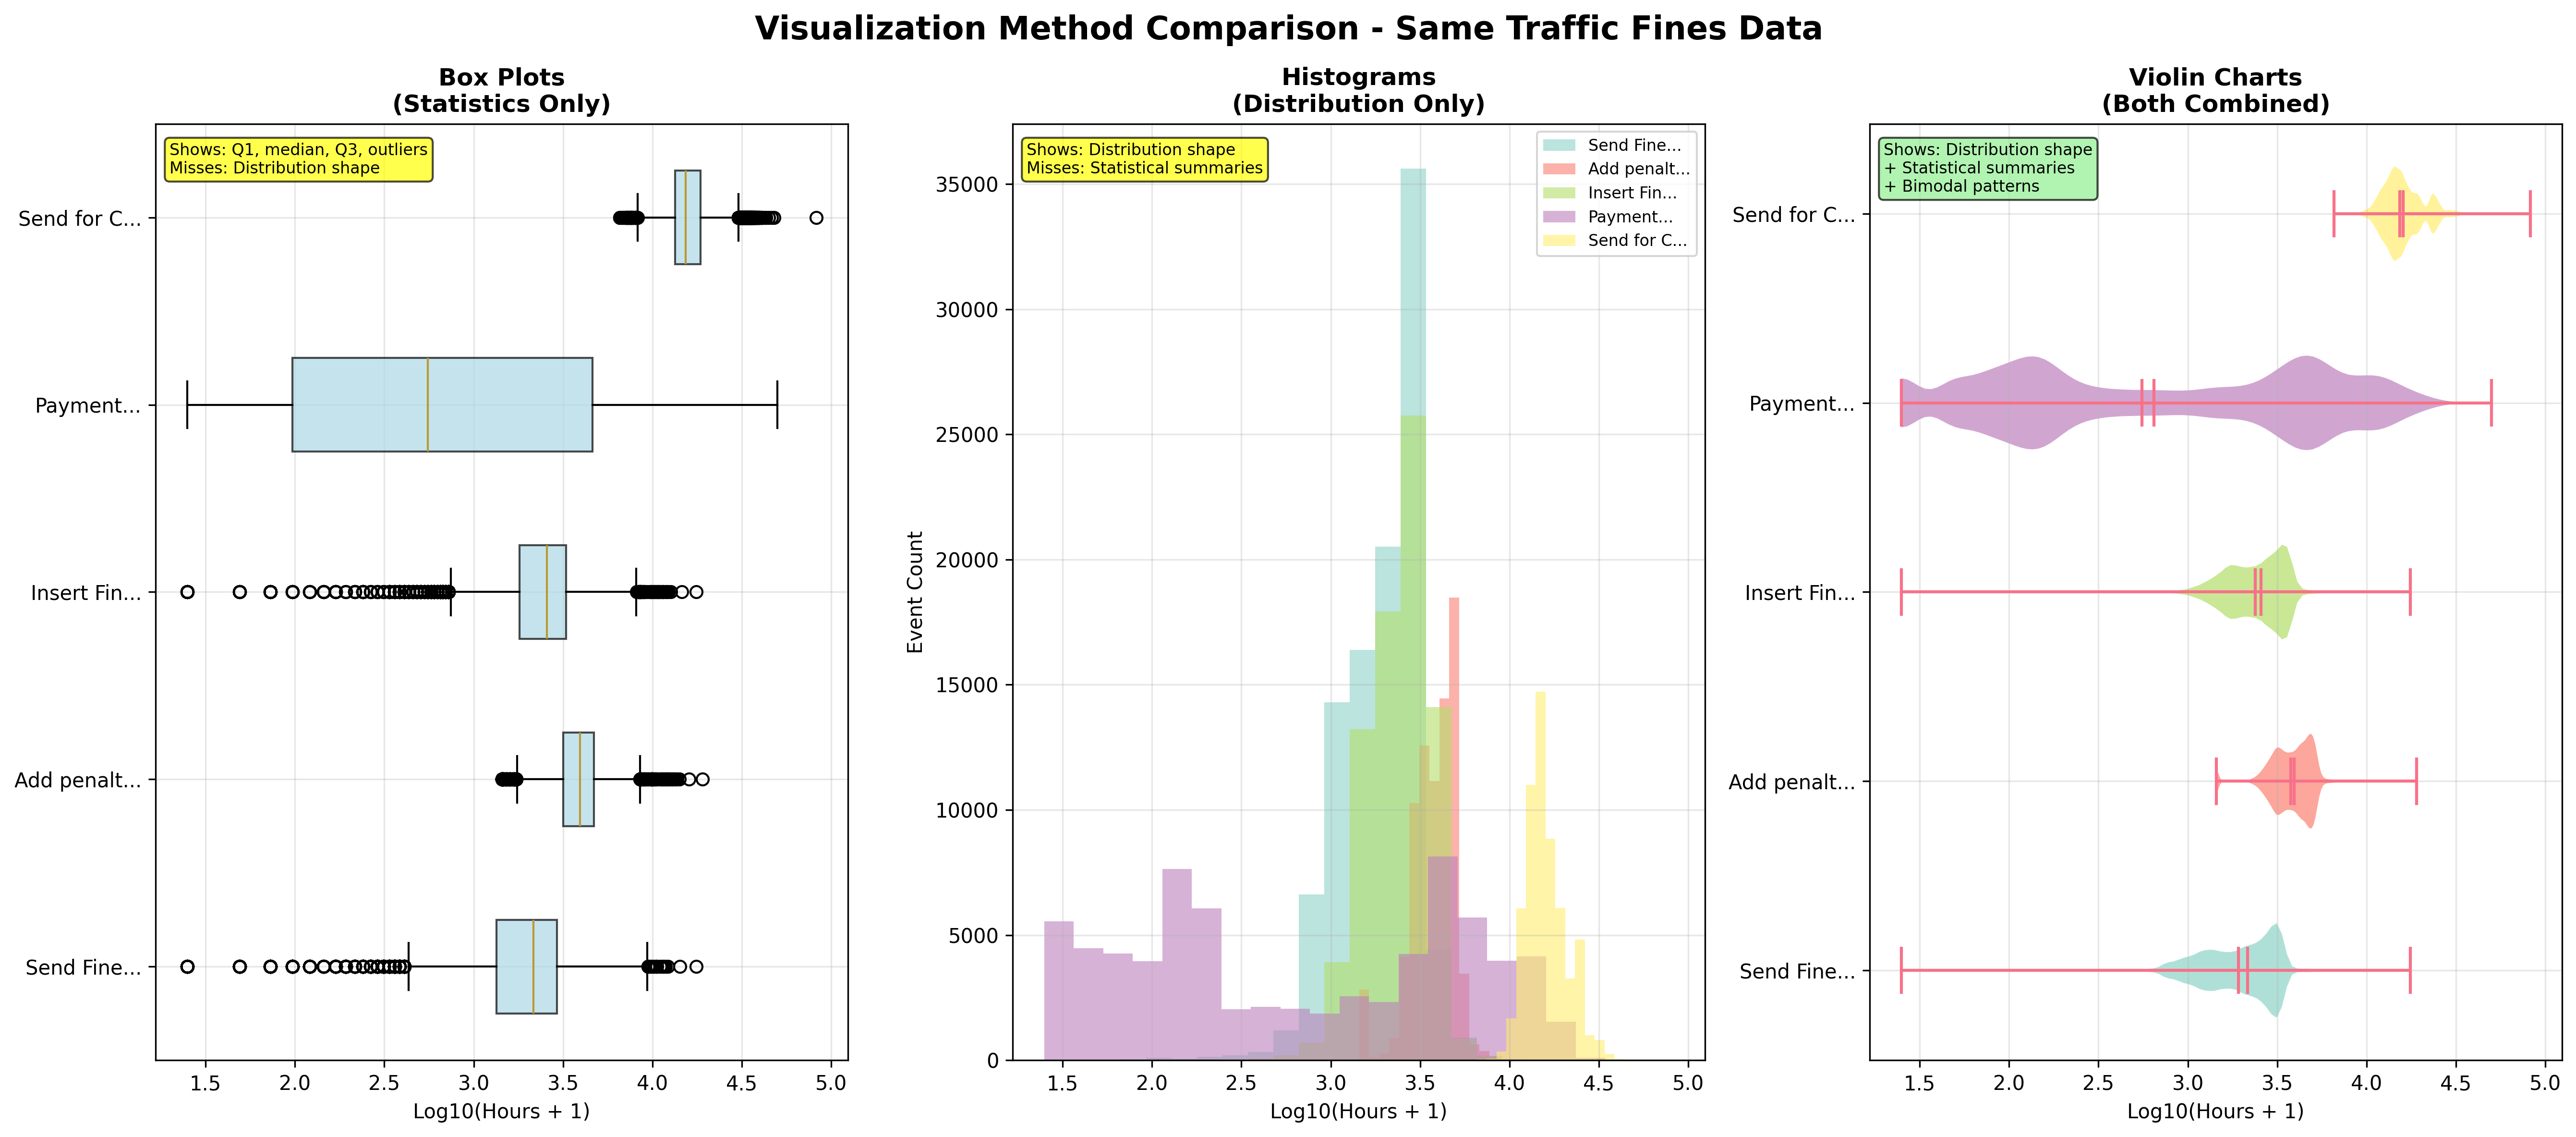
\includegraphics[width=\textwidth]{fig/violin_vs_traditional.png}
\caption{Comparison of visualization methods for the same Traffic Fines data. Box plots show statistical summaries but miss distribution shape, histograms show distribution but hide statistics, while violin charts integrate both perspectives to reveal bimodal patterns and statistical summaries simultaneously.}
\label{fig:violin_vs_traditional}
\end{figure}

\textbf{Multimodal Patterns:} Traffic Fines showed clear bimodal distributions indicating two distinct citizen behavior patterns (immediate vs delayed payment), information lost in box plots or histograms.

\textbf{Distribution Shapes:} Healthcare processes exhibited left-skewed distributions reflecting urgent care protocols, while financial processes showed right-skewed patterns indicating processing delays.

\textbf{Statistical Integration:} Simultaneous display of distribution shape and statistical summaries enabled comprehensive analysis without switching between multiple chart types.

\textbf{Interactive Exploration:} Different statistical sorting revealed complementary insights - frequency sorting identified common events while mean sorting revealed typical timing patterns, as shown in Figure \ref{fig:sorting_effects}.

\begin{figure}[H]
\centering
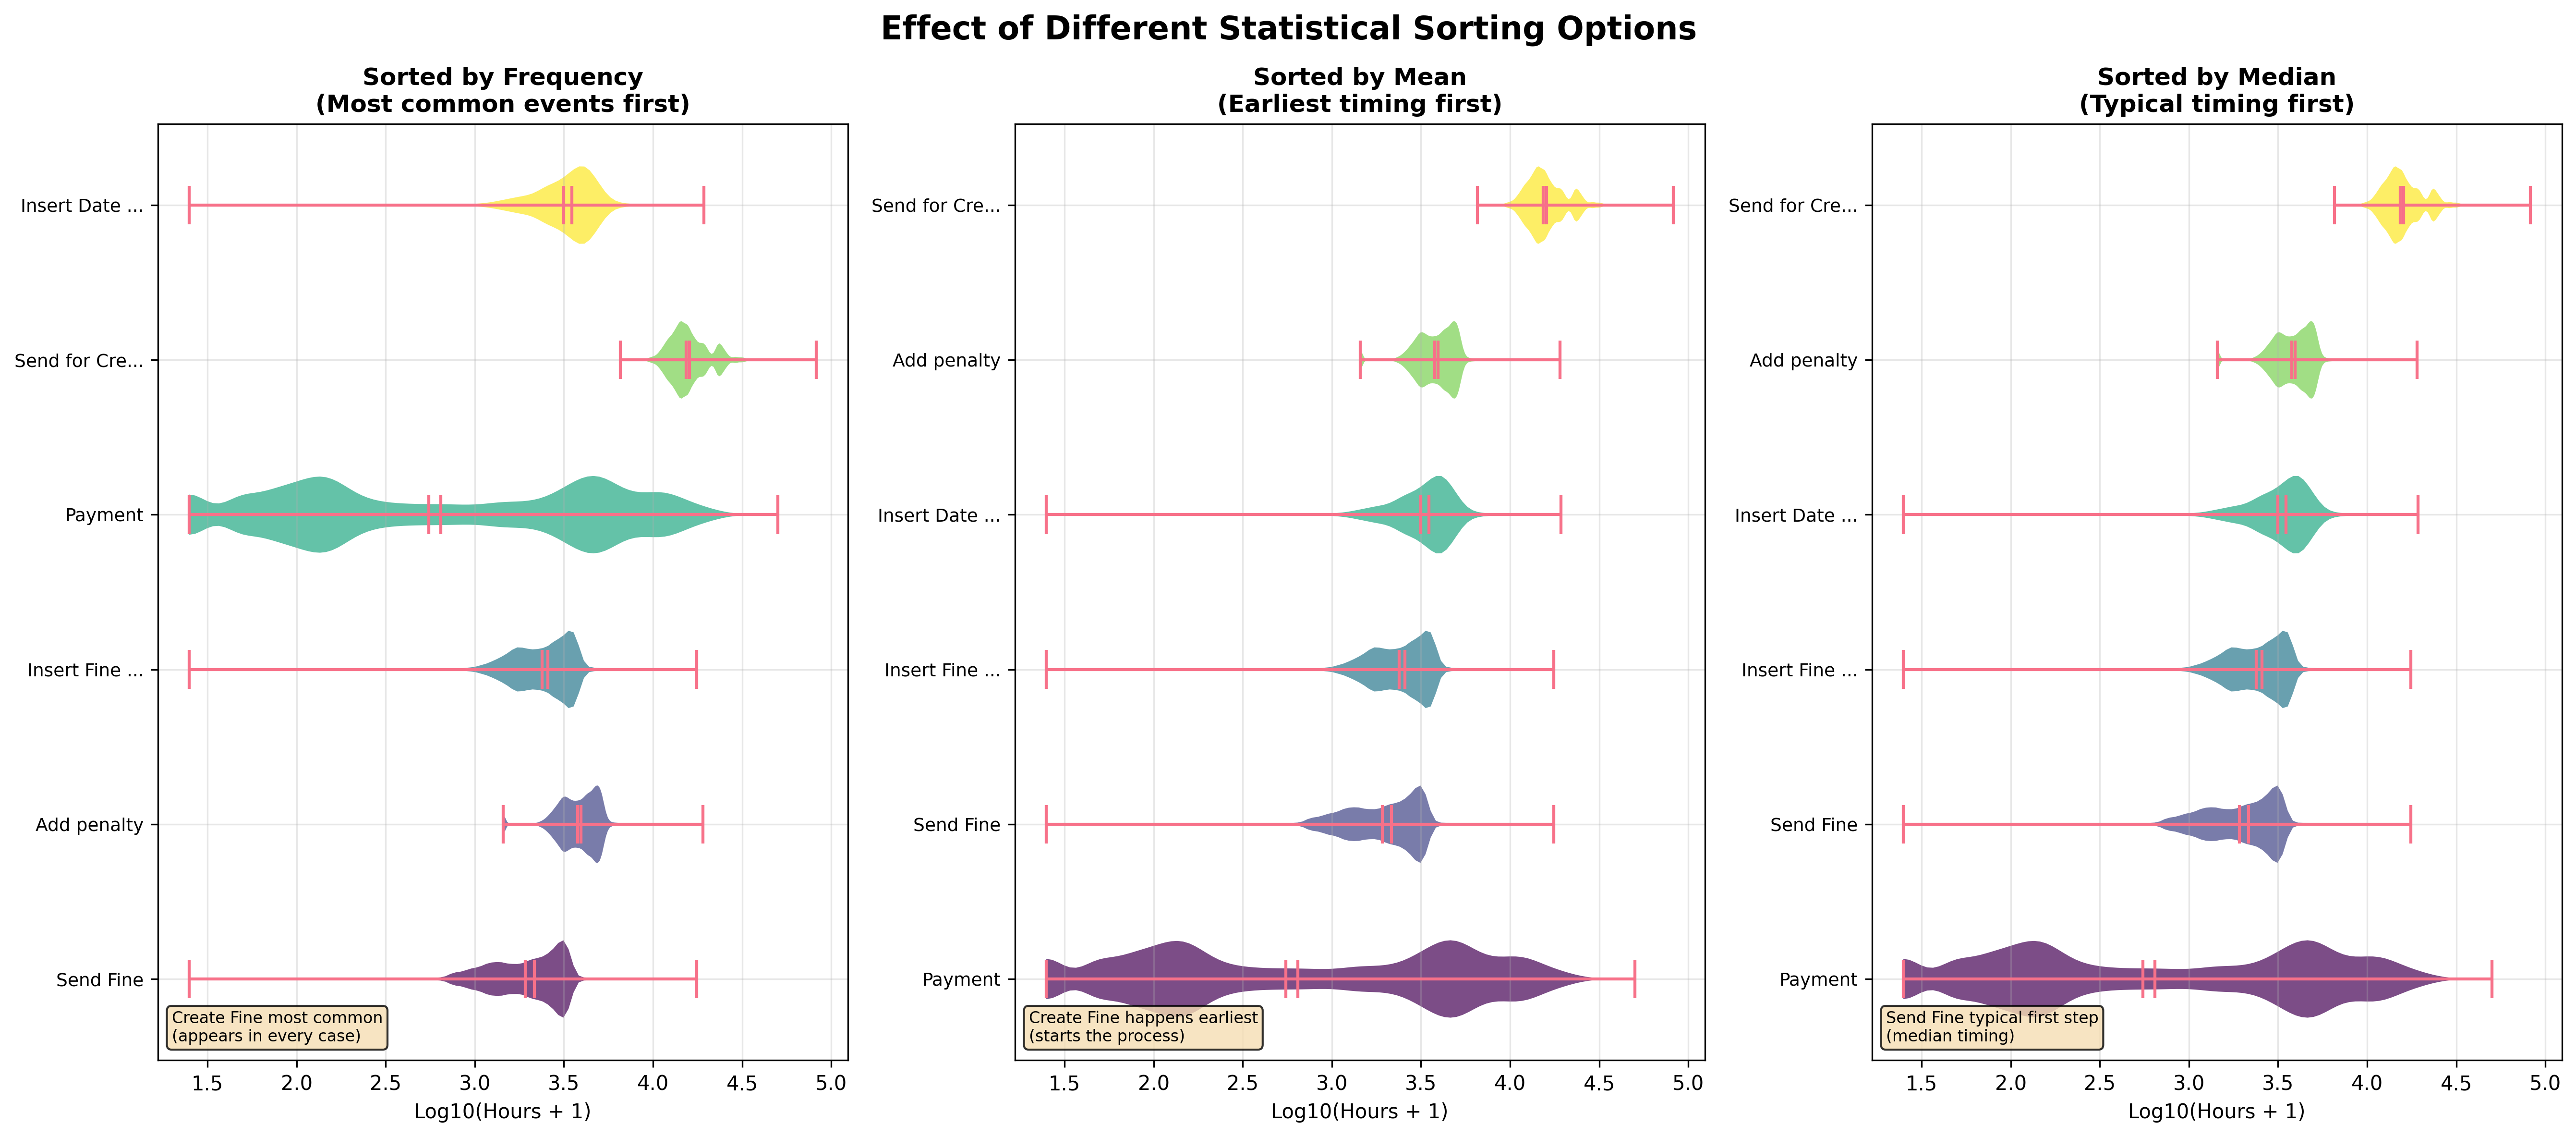
\includegraphics[width=\textwidth]{fig/sorting_effects.png}
\caption{Effect of different statistical sorting options on event ordering. Frequency sorting reveals the most common events, mean sorting shows which events typically occur early or late, and median sorting highlights typical timing patterns. Each perspective provides different analytical insights from the same data.}
\label{fig:sorting_effects}
\end{figure}

\subsection{Limitations and Discussion}
\label{subsec:limitations}

Several limitations emerged during evaluation:

\textbf{Sparse Data Handling:} Very sparse distributions with few events can create misleading violin shapes. Our minimum event threshold of 100 occurrences helps but doesn't eliminate this issue.

\textbf{Extreme Outliers:} Despite filtering and transformation, some datasets still contain extreme outliers that can distort visualizations. Manual outlier detection may be needed for certain analyses.

\textbf{Transformation Selection:} Users need domain knowledge to select optimal transformations. Automatic transformation recommendation could improve usability.

\textbf{Scalability Limits:} While tested up to 1.2 million events, performance with datasets exceeding 10 million events remains unknown and may require additional optimization.

Despite these limitations, the approach successfully addresses the core requirements and provides significant improvements over traditional visualization methods for process mining analysis.

% =====================================================================================
% SECTION 5: CONCLUSION
% =====================================================================================

\section{Conclusion}
\label{sec:conclusion}

This paper presents a comprehensive approach to visualizing event type distributions over time in process mining through interactive violin charts. Our implementation successfully addresses key challenges in temporal event analysis by combining statistical summaries with distribution shapes in a single, interpretable visualization.

\subsection{Key Contributions}
\label{subsec:contributions}

Our work makes several important contributions to process mining visualization:

\textbf{Integrated Visualization Design:} We developed violin charts that simultaneously display distribution shapes and statistical summaries, eliminating the need to switch between multiple visualization types. This integration enables analysts to identify patterns such as bimodal distributions while maintaining access to quantitative measures.

\textbf{Flexible Time Transformation Framework:} Our approach provides multiple transformation options (logarithmic, square root, raw, and min-max scaling) that adapt to different dataset characteristics. This flexibility proves essential as no single transformation works optimally across all process domains and timing scales.

\textbf{Cross-Domain Pattern Discovery:} Testing across government, finance, and healthcare processes revealed distinct temporal signatures for each domain. Government processes exhibit regulatory deadline patterns, financial processes show structured workflow stages, and healthcare processes demonstrate time-critical clustering.

\textbf{Event Filtering:} Our case-start event filtering preserves analytical validity while removing noise that obscures meaningful patterns. The filtering effectiveness varies by process structure, with simpler processes showing higher filtering rates.

\textbf{Interactive Statistical Sorting:} Multiple sorting options (frequency, mean, median) provide complementary analytical perspectives from the same data, enabling comprehensive exploration of timing patterns.

\subsection{Practical Impact}
\label{subsec:impact}

The evaluation demonstrates significant practical benefits over traditional visualization approaches:

\textbf{Pattern Recognition:} Complex patterns like bimodal distributions in government processes and time-critical clustering in healthcare are clearly visible, information that remains hidden in box plots or histograms.

\textbf{Process Understanding:} The visualization reveals domain-specific timing behaviors, such as citizen payment patterns in traffic fines (30-day and 6-month peaks) and clinical protocol adherence in sepsis treatment.

\textbf{Analytical Efficiency:} Single-view access to both statistical and distributional information reduces cognitive load and analysis time compared to examining multiple separate charts.

\textbf{Scalability:} The approach handles datasets ranging from 15,000 to 1.2 million events while maintaining interactive performance and visual clarity.

\subsection{Limitations and Future Work}
\label{subsec:future}

Several limitations suggest directions for future research:


\textbf{Sparse Data Visualization:} Event types with very few occurrences can create misleading violin shapes. Advanced smoothing techniques or alternative visualization methods for sparse data merit investigation.

\textbf{Scalability Boundaries:} While tested up to 1.2 million events, performance with datasets exceeding 10 million events remains unexplored and may require additional optimization strategies.

\textbf{Comparative Analysis Tools:} Enhanced support for cross-dataset comparison could provide deeper insights into process mining patterns across different domains and organizations.

\subsection{Final Remarks}
\label{subsec:remarks}

Our approach demonstrates that violin charts provide a powerful tool for temporal event analysis in process mining. The combination of distribution visualization, statistical integration, and flexible transformation makes complex timing patterns accessible to analysts across diverse domains. The cross-domain evaluation validates the approach's generalizability while revealing domain-specific insights that inform both research and practice.

The implementation provides a solid foundation for future process mining visualization research, particularly in temporal analysis and cross-domain pattern discovery. As process mining continues to expand across industries, visualization tools that adapt to diverse timing characteristics while maintaining analytical rigor become increasingly important for extracting actionable insights from complex event data.


\bibliographystyle{plain}
\bibliography{references}

\end{document}
